%  LaTeX support: latex@mdpi.com
%  In case you need support, please attach all files that are necessary for compiling as well as the log file, and specify the details of your LaTeX setup (which operating system and LaTeX version / tools you are using).

%=================================================================
\documentclass[Dance Data
Project,article,submit,moreauthors,pdftex]{mdpi}

% If you would like to post an early version of this manuscript as a preprint, you may use preprint as the journal and change 'submit' to 'accept'. The document class line would be, e.g., \documentclass[preprints,article,accept,moreauthors,pdftex]{mdpi}. This is especially recommended for submission to arXiv, where line numbers should be removed before posting. For preprints.org, the editorial staff will make this change immediately prior to posting.

%% Some pieces required from the pandoc template
\setlist[itemize]{leftmargin=*,labelsep=5.8mm}
\setlist[enumerate]{leftmargin=*,labelsep=4.9mm}


%--------------------
% Class Options:
%--------------------
%----------
% journal
%----------
% Choose between the following MDPI journals:
% acoustics, actuators, addictions, admsci, aerospace, agriculture, agriengineering, agronomy, algorithms, animals, antibiotics, antibodies, antioxidants, applsci, arts, asc, asi, atmosphere, atoms, axioms, batteries, bdcc, behavsci , beverages, bioengineering, biology, biomedicines, biomimetics, biomolecules, biosensors, brainsci , buildings, cancers, carbon , catalysts, cells, ceramics, challenges, chemengineering, chemistry, chemosensors, children, cleantechnol, climate, clockssleep, cmd, coatings, colloids, computation, computers, condensedmatter, cosmetics, cryptography, crystals, dairy, data, dentistry, designs , diagnostics, diseases, diversity, drones, econometrics, economies, education, electrochem, electronics, energies, entropy, environments, epigenomes, est, fermentation, fibers, fire, fishes, fluids, foods, forecasting, forests, fractalfract, futureinternet, futurephys, galaxies, games, gastrointestdisord, gels, genealogy, genes, geohazards, geosciences, geriatrics, hazardousmatters, healthcare, heritage, highthroughput, horticulturae, humanities, hydrology, ijerph, ijfs, ijgi, ijms, ijns, ijtpp, informatics, information, infrastructures, inorganics, insects, instruments, inventions, iot, j, jcdd, jcm, jcp, jcs, jdb, jfb, jfmk, jimaging, jintelligence, jlpea, jmmp, jmse, jnt, jof, joitmc, jpm, jrfm, jsan, land, languages, laws, life, literature, logistics, lubricants, machines, magnetochemistry, make, marinedrugs, materials, mathematics, mca, medicina, medicines, medsci, membranes, metabolites, metals, microarrays, micromachines, microorganisms, minerals, modelling, molbank, molecules, mps, mti, nanomaterials, ncrna, neuroglia, nitrogen, notspecified, nutrients, ohbm, particles, pathogens, pharmaceuticals, pharmaceutics, pharmacy, philosophies, photonics, physics, plants, plasma, polymers, polysaccharides, preprints , proceedings, processes, proteomes, psych, publications, quantumrep, quaternary, qubs, reactions, recycling, religions, remotesensing, reports, resources, risks, robotics, safety, sci, scipharm, sensors, separations, sexes, signals, sinusitis, smartcities, sna, societies, socsci, soilsystems, sports, standards, stats, surfaces, surgeries, sustainability, symmetry, systems, technologies, test, toxics, toxins, tropicalmed, universe, urbansci, vaccines, vehicles, vetsci, vibration, viruses, vision, water, wem, wevj

%---------
% article
%---------
% The default type of manuscript is "article", but can be replaced by:
% abstract, addendum, article, benchmark, book, bookreview, briefreport, casereport, changes, comment, commentary, communication, conceptpaper, conferenceproceedings, correction, conferencereport, expressionofconcern, extendedabstract, meetingreport, creative, datadescriptor, discussion, editorial, essay, erratum, hypothesis, interestingimages, letter, meetingreport, newbookreceived, obituary, opinion, projectreport, reply, retraction, review, perspective, protocol, shortnote, supfile, technicalnote, viewpoint
% supfile = supplementary materials

%----------
% submit
%----------
% The class option "submit" will be changed to "accept" by the Editorial Office when the paper is accepted. This will only make changes to the frontpage (e.g., the logo of the journal will get visible), the headings, and the copyright information. Also, line numbering will be removed. Journal info and pagination for accepted papers will also be assigned by the Editorial Office.

%------------------
% moreauthors
%------------------
% If there is only one author the class option oneauthor should be used. Otherwise use the class option moreauthors.

%---------
% pdftex
%---------
% The option pdftex is for use with pdfLaTeX. If eps figures are used, remove the option pdftex and use LaTeX and dvi2pdf.

%=================================================================
\firstpage{1}
\makeatletter
\setcounter{page}{\@firstpage}
\makeatother
\pubvolume{xx}
\issuenum{1}
\articlenumber{5}
\pubyear{2019}
\copyrightyear{2019}
%\externaleditor{Academic Editor: name}
\history{Received: date; Accepted: date; Published: date}
\updates{yes} % If there is an update available, un-comment this line

%% MDPI internal command: uncomment if new journal that already uses continuous page numbers
%\continuouspages{yes}

%------------------------------------------------------------------
% The following line should be uncommented if the LaTeX file is uploaded to arXiv.org
%\pdfoutput=1

%=================================================================
% Add packages and commands here. The following packages are loaded in our class file: fontenc, calc, indentfirst, fancyhdr, graphicx, lastpage, ifthen, lineno, float, amsmath, setspace, enumitem, mathpazo, booktabs, titlesec, etoolbox, amsthm, hyphenat, natbib, hyperref, footmisc, geometry, caption, url, mdframed, tabto, soul, multirow, microtype, tikz

%=================================================================
%% Please use the following mathematics environments: Theorem, Lemma, Corollary, Proposition, Characterization, Property, Problem, Example, ExamplesandDefinitions, Hypothesis, Remark, Definition
%% For proofs, please use the proof environment (the amsthm package is loaded by the MDPI class).

%=================================================================
% Full title of the paper (Capitalized)
\Title{Analysis of Dance Data Company Endowments, Assetes, and Labor in
the United States}

% Authors, for the paper (add full first names)
\Author{Rose
Evard$^{1}$\href{https://orcid.org/0000-0003-3293-2315}{\orcidicon}, Ruth
Button$^{1}$, Zhen
Nie$^{1}$\href{https://orcid.org/0009-0009-3690-4953}{\orcidicon}, Quinn
White$^{1}$\href{https://orcid.org/0000-0001-5399-0237}{\orcidicon}}

% Authors, for metadata in PDF
\AuthorNames{Rose Evard, Ruth Button, Zhen Nie, Quinn White}

% Affiliations / Addresses (Add [1] after \address if there is only one affiliation.)
\address{%
$^{1}$ \quad Smith College Statistical \& Data Sciences Department 1
Chapin Way, Northampton, MA, 01063; \\
}
% Contact information of the corresponding author
\corres{Correspondence: \href{mailto:andrew.hoekstra@dancedataproject.com}{\nolinkurl{andrew.hoekstra@dancedataproject.com}}}

% Current address and/or shared authorship
\firstnote{Current address: Updated affiliation}
\secondnote{These authors contributed equally to this work.}






% The commands \thirdnote{} till \eighthnote{} are available for further notes

% Simple summary

% Abstract (Do not insert blank lines, i.e. \\)
\abstract{To understand how we can advance equity in dance, it is
crucial to understand existing financial structures and incentives that
shape these companies' success. Assessment of publicly available tax
documents on dance companies over the past decade can provide important
insights into how different companies fared financially over this time
period. Additionally, this work can provide an important basis of
understanding for future analyses on the impact of the pandemic on
existing trends on the financial performance. By analyzing publicly
available Form 990 documents on 169 dance companies across the United
States, we present information on companies' endowments, investments,
compensation of employees, and sources of labor. In the process, we also
bring light to issues of data quality to consider when analyzing Form
990 documents.}

% Keywords
\keyword{Endowment; Non-Profit; Volunteer Labor; Dance.}

% The fields PACS, MSC, and JEL may be left empty or commented out if not applicable
%\PACS{J0101}
%\MSC{}
%\JEL{}

%%%%%%%%%%%%%%%%%%%%%%%%%%%%%%%%%%%%%%%%%%
% Only for the journal Diversity
%\LSID{\url{http://}}

%%%%%%%%%%%%%%%%%%%%%%%%%%%%%%%%%%%%%%%%%%
% Only for the journal Applied Sciences:
%\featuredapplication{Authors are encouraged to provide a concise description of the specific application or a potential application of the work. This section is not mandatory.}
%%%%%%%%%%%%%%%%%%%%%%%%%%%%%%%%%%%%%%%%%%

%%%%%%%%%%%%%%%%%%%%%%%%%%%%%%%%%%%%%%%%%%
% Only for the journal Data:
%\dataset{DOI number or link to the deposited data set in cases where the data set is published or set to be published separately. If the data set is submitted and will be published as a supplement to this paper in the journal Data, this field will be filled by the editors of the journal. In this case, please make sure to submit the data set as a supplement when entering your manuscript into our manuscript editorial system.}

%\datasetlicense{license under which the data set is made available (CC0, CC-BY, CC-BY-SA, CC-BY-NC, etc.)}

%%%%%%%%%%%%%%%%%%%%%%%%%%%%%%%%%%%%%%%%%%
% Only for the journal Toxins
%\keycontribution{The breakthroughs or highlights of the manuscript. Authors can write one or two sentences to describe the most important part of the paper.}

%\setcounter{secnumdepth}{4}
%%%%%%%%%%%%%%%%%%%%%%%%%%%%%%%%%%%%%%%%%%


% tightlist command for lists without linebreak
\providecommand{\tightlist}{%
  \setlength{\itemsep}{0pt}\setlength{\parskip}{0pt}}

% From pandoc table feature
\usepackage{longtable,booktabs,array}
\usepackage{calc} % for calculating minipage widths
% Correct order of tables after \paragraph or \subparagraph
\usepackage{etoolbox}
\makeatletter
\patchcmd\longtable{\par}{\if@noskipsec\mbox{}\fi\par}{}{}
\makeatother
% Allow footnotes in longtable head/foot
\IfFileExists{footnotehyper.sty}{\usepackage{footnotehyper}}{\usepackage{footnote}}
\makesavenoteenv{longtable}


\usepackage{caption}
\captionsetup[figure]{font=scriptsize}
\usepackage{booktabs}
\usepackage{longtable}
\usepackage{array}
\usepackage{multirow}
\usepackage{wrapfig}
\usepackage{float}
\usepackage{colortbl}
\usepackage{pdflscape}
\usepackage{tabu}
\usepackage{threeparttable}
\usepackage{threeparttablex}
\usepackage[normalem]{ulem}
\usepackage{makecell}
\usepackage{xcolor}

\begin{document}


%%%%%%%%%%%%%%%%%%%%%%%%%%%%%%%%%%%%%%%%%%

\hypertarget{introduction}{%
\section{Introduction}\label{introduction}}

\hypertarget{scope}{%
\subsection{Scope}\label{scope}}

As a matter of transparency and public accountability, tax documents
filed by nonprofit corporations in the United States have always
theoretically been available to the public, but it wasn't until the
development of electronic tax filing systems through the IRS that these
tax documents became easily accessible for analysis. Online tax filing
systems have been available since the late 1990's, but the 2019 Taxpayer
First Act required all nonprofits to electronically file their tax
returns (Ely et al., 2023). This legislation changed the landscape for
public accessibility of the financial information of nonprofits as well
as presented novel research opportunities for data activism. Incorrect
reporting, inequitable wealth distribution, and tax fraud by nonprofit
organizations has always happened, but mandatory online reporting allows
data analysts to identify suspected cases and draw attention to them
(Ely et al., 2023).

\hypertarget{inequality-in-the-arts}{%
\subsection{Inequality in the Arts}\label{inequality-in-the-arts}}

The study of women and gender has consistently drawn focus to
inequitable distribution of wealth between men and women. One of the
most heavily researched phenomena regarding wealth inequality is the
wage gap between men and women that persists even when they have the
same education, experience, skills, and job titles (Jikar, 2022).
Contrary to the popular opinion that the gender wage gap is narrowing,
Weichselbaumer \& Winter-Ebmer (2005) showed that financial returns in
relation to skills and education are increasingly higher for men than
for women. Even less research has been done on the wage gap for
transgender or non-binary individuals. Additionally, compounding factors
such as lack of corporate oversight and socially-imposed gender roles
further entrench the gender pay gap into everyday life (Pub, 2013).
Further understanding the wage gap in female-dominated fields, such as
in dance, can inform future solutions to lessen the inequitable
distribution of wealth between men and women.

The wage gap has long been exacerbated by disproportionate pay in the
arts, and especially dance, in part because the vast majority of
entry-level dancers are women and girls (Jikar, 2022). Additionally,
unpaid labor in dance is much more commonplace than in other industries
(Pub, 2013). Because dance is a performing art, many companies that
employ dancers are entitled to government subsidies and tax breaks;
however, there are no current regulations to ensure that this
governmental assistance is used to lessen unpaid and underpaid labor by
dancers (Fuchs, 2021). Unrestricted financial assistance may worsen
existing inequalities in the field of dance by enabling company owners
and executives to profit while retaining unpaid and underpaid labor, so
further understanding how this assistance is used is essential in
combating the problem.

\hypertarget{dance-and-tax-returns}{%
\subsection{Dance and Tax Returns}\label{dance-and-tax-returns}}

In the United States, nonprofit organizations file either a Form 900 or
a Form 990 EZ with the IRS each year. These documents include, but are
not limited to, information on the organization's geographic location,
number of employees and volunteers, operating costs, income,
compensation, and net assets. This information is more accessible than
ever now that the government has required nonprofit organizations to
electronically file them. Yet, much of the public does not understand
the terms on publicly available tax forms nor does the average person
possess the skills to readily analyze hundreds of tax forms every year
(Lamonthe, 2023). Thus, data scientists can play a very important role
in analyzing these forms filed by dance companies and presenting
findings to the public. Further elucidating the financial practices of
nonprofit organizations 1) in the field of dance, 2) in pandemic-related
economic shifts and 3) through geographical analysis can help inform
proper solutions to a wide range of issues, including the gender pay gap
in dance.

\hypertarget{the-dance-data-project}{%
\subsection{The Dance Data Project}\label{the-dance-data-project}}

We completed this project in collaboration with our project sponsor, the
Dance Data Project (also known as the DDP). The Dance Data Project is a
non-profit organization dedicated to equality in the arts. Founded in
2015 by former ballet dancer and philanthropist Elizabeth Yntema, the
DDP uses data and research to promote transparency, accountability, and
action towards gender equality in dance.

The DDP collects, analyzes, and presents data to outline lack of
leadership opportunities for female directors, choreographers,
composers, set, costume, lighting designers, and back-of-house positions
in dance. The organization seeks to create a world where all dancers,
regardless of gender, race, ethnicity, or socioeconomic status, have
equal access to opportunities and resources in the dance world. The
organization also advocates for removing barriers for female employment
and advancement in this industry, such as lack of parental and elder
leave, day care system, and protocol for sexual harassment by presenting
their findings on television news such as MSNBC and publishing articles
in magazines such as \emph{Vogue} and \emph{People}. Through its
data-driven research, advocacy, and education efforts, the DDP works to
create a more equitable and inclusive dance community where all
individuals have the opportunity to pursue their passion for dance.

\hypertarget{scope-1}{%
\subsection{Scope}\label{scope-1}}

This project will be a preliminary analysis of publicly available
financial information on dance companies in the United States. Results
will be collected for and shared with Dance Data Project for any
publications or future analyses that they perform. Because little
analysis has been done on financial practices of dance companies in the
United States, our exploratory approach will examine broad research
areas regarding how dance companies manage endowments, employment, and
properties.

The bulk of our report consists of examining how companies' financial
resources (particularly endowments) behave over time, in comparison to
one another, and in comparison to the S\&P 500. We also look into the
use of volunteer labor alongside the use of paid employment labor and
how geographical location impacts the use of each type of labor.

The data source for this project is a collection of IRS Form 990's and
IRS Form 990 EZ's from dance companies in the United States. These
publicly available tax documents are required annual filings for
nonprofits\footnote{Most major dance companies are nonprofits.} {]}and
include information including each the number of employees and
volunteers, compensation to employees, geographical location, and annual
revenue. We primarily present analysis based on Schedule D of the Form
990. Only companies meeting certain criteria regarding the possession of
certain funds and assets must file Schedule D, which contains data on
endowment funds as well as building values and other assets. Our
analysis seeks to capture trends in how these companies have managed
their assets and endowments, primarily in the time span of 2014 to 2020,
with the goal of bringing transparency to the financial side of the
dance industry.

\hypertarget{ethics-statement}{%
\section{Ethics Statement}\label{ethics-statement}}

This project included signing a non-disclosure agreement with Dance Data
Project in which each group member agreed to keep specific collections
of data produced by DDP confidential. Still, data that was collected
during our analyses was not covered by the NDA but was still sensitive.
The potential impact of this information getting into the wrong hands
would be harmful to the Dance Data Project and their ability to publish
the findings. Certain information could be used by dance companies to
silence the DDP's message or competitors could publish and get
recognition for DDP's proprietary information. Therefore, each team
member was especially careful not to disclose any information that may
harm DDP's work to third parties.

We also assumed that data reported on the IRS 990, 990EZ, and Schedule D
forms was accurate unless identifiable discrepancies were found or
amendments were reported. The social harm that could occur from this
assumption is dance companies who accidentally misreport on their tax
documents may be identified in our analyses as violating ethical or
financial norms. In order to prevent this, our team and DDP collaborated
to reach out to companies to ask for clarification of our findings
before potentially publishing their name.

Finally, all of us have training in data science, but we are not
dancers. Because none of us have lived experience in dance, we cannot
provide personal expertise in analyzing this data. Additionally, our
group all identifies as female and none of us are Black. The standpoints
of dancers, men, and people of diverse backgrounds in data analyses may
offer a more comprehensive understanding of the context behind our
dataset. In order to reduce our bias (although it was not possible to
change our social identities), we spoke with our project sponsors about
how to approach this data that may impact other social groups.

\hypertarget{detailed-methodology}{%
\section{Detailed Methodology}\label{detailed-methodology}}

\hypertarget{data-acquisition}{%
\subsection{Data Acquisition}\label{data-acquisition}}

Data files were gathered by Andrew Hoekstra, data consultant from DDP,
prior to February 8th, 2022 from publicly available IRS APIs. Form 990s
were downloaded as XMLs. Our sample contained 169 US dance companies in
total, with Form 990s submitted between 2015 and 2022, thus representing
fiscal years 2014 through 2021. For Schedule D in particular, companies
are required to report endowment totals up to 4 fiscal years prior, thus
our endowment data spans 2010 to 2021.

\hypertarget{initial-wrangling-filtering}{%
\subsection{Initial Wrangling \&
Filtering}\label{initial-wrangling-filtering}}

Form 990 can be completed in three different formats: Form 990, Form
900-EZ, and Form 990-T. We excluded all Form 990-Ts because these forms
do not contain relevant information on variables considered in our
analyses. Additionally, when a company amended a filing, and hence had
multiple filings corresponding to a single fiscal year, we took the
amended filing.

\hypertarget{company-communication}{%
\subsection{Company Communication}\label{company-communication}}

Because companies report data across years, a useful data quality check
can be if the year they reported for the previous years in a filing
correspond to the values they actually reported in those years.

For example, when a company reports in their 2020 filing the beginning
of year endowment balance for years 2016 through 2020, we can check
whether the value they reported for 2016 in 2020 was indeed what they
reported in 2016. Reporting was highly consistent across the companies
considered; however, there were some notable discrepancies, particularly
in earlier years. When we identified these discrepancies, we reached out
to the companies to clarify which values were correct. We received
prompt responses from BalletMet and Pittsburgh Ballet, who confirmed the
more recently reported values were correct.

Because discrepancies were typically in earlier years, and our
communications with the companies who did respond noted their most
recently reported values were correct, in our analyses we took the most
recent data available. For example, we took values for 2016-2020 from
the 2020 filing instead of taking the current year values for the filing
from each year separately.

Another result of this approach is that we can look back through 2010 in
some cases, since although we only have filings that go back to 2014,
each filing has data going back four years.

\hypertarget{standard-definitions}{%
\subsection{Standard Definitions}\label{standard-definitions}}

\begin{longtable}[]{@{}
  >{\raggedright\arraybackslash}p{(\columnwidth - 2\tabcolsep) * \real{0.3889}}
  >{\raggedright\arraybackslash}p{(\columnwidth - 2\tabcolsep) * \real{0.6111}}@{}}
\toprule()
\begin{minipage}[b]{\linewidth}\raggedright
Term
\end{minipage} & \begin{minipage}[b]{\linewidth}\raggedright
Definition
\end{minipage} \\
\midrule()
\endhead
Endowment & The form 990 uses the definition of the endowment (and types
of endowments) from the
\href{https://asc.fasb.org/MasterGlossary}{Financial Accounting
Standards Board}, which defines an endowment fund as ``An established
fund of cash, securities, or other assets to provide income for the
maintenance of a not-for-profit entity (NFP). The use of the assets of
the fund may be with or without donor-imposed restrictions.'' \\
Rank & \\
Percent Change & The percent change is
\(\frac{\text{End Value} - \text{Beginning Value}}{\text{Beginning Value}} \times 100.\) \\
S\&P 500 & The Standard and Poor's 500 Index is a standard index used as
a benchmark to describe the behavior of the stock market overall. The
index includes 500 top publicly traded companies and is weighted by the
market value of stocks currently held by stakeholders, where companies
with higher market value receive higher weight. \\
Compound Annual Growth Rate & The compound growth rate (CAGR) describes
a company's average growth over multiple years. It is useful as a
smoothed metric to look over growth over a set of years and compare
companies in the same time period. For a time period of \(t\) years, we
compute the annual growth rate as
\({\text{Compound Annual Growth Rate} = \left( \frac{\text{End Value}}{\text{Beginning Value}}\right)^{\frac{1}{\text{End Year} - \text{Beginning Year}}}-1}\). \\
\bottomrule()
\end{longtable}

\hypertarget{findings}{%
\section{Findings}\label{findings}}

\hypertarget{endowments}{%
\subsection{Endowments}\label{endowments}}

\href{https://www.investopedia.com/terms/e/endowment.asp}{Endowments}
are donated funds to nonprofit organizations which are invested.
Endowments are typically designed to maintain initial donations
(principal funds); the investment income produced by the invested
donation can be utilized for specific purposes. Depending on endowment
management and policies, some organizations can remove a certain amount
of principal assets from their endowment per year.

\hypertarget{types-of-endowments}{%
\subsubsection{Types of Endowments}\label{types-of-endowments}}

There are \href{https://www.irs.gov/instructions/i990sd}{three
categories} of endowment funds as defined by the IRS.

\begin{itemize}
\tightlist
\item
  \textbf{Term endowments}(temporarily restricted endowments) are funds
  that are donor-restricted, which means they are meant to be used for a
  certain amount of time or until a particular event.
\item
  \textbf{Permanent endowments} are endowment funds from
  donor-restricted gifts where the initial fund must be invested;
  however gains or losses from these investments can be used by the
  organization.\\
\item
  \textbf{Board-designated or quasi-endowment} are funds that were
  internally designated for specific use but are not donor-restricted.
  Investment gains and losses are typically utilized; however, the
  principal funds can be expended at any time.
\end{itemize}

Most dance companies have their endowment funds primarily in the
permanent endowment category, whereas the proportion held as a board
designated/quasi-endowment is typically less than 25\%, as is the
proportion held as a temporarily restricted endowment
(\ref{fig:endowment-type}). For the majority of companies, the
proportions held in each category are fairly consistent across the
years. In fact, some companies held their endowment in a single category
across all years on file (Table \ref{table:endowment-type-table}).

\begin{table}

\caption{Organizations with $100\%$ of their Endowments in One Category for All Years on File}
\centering
\begin{tabular}[t]{l>{\raggedleft\arraybackslash}p{4cm}}
\toprule
Organization Name & Number of Years on File\\
\midrule
\addlinespace[0.5em]
\multicolumn{2}{l}{\textbf{Board designated or quasi-endowment}}\\
\hline
\hspace{1em}The Tallahassee Ballet & 6\\
\hspace{1em}Ballet Quad Cities & 2\\
\hspace{1em}Canyon Concert Ballet & 1\\
\addlinespace[0.5em]
\multicolumn{2}{l}{\textbf{Permanent endowment}}\\
\hline
\hspace{1em}Pittsburgh Ballet Theatre & 7\\
\hspace{1em}Dance Theatre of Harlem, Madison Ballet & 6\\
\hspace{1em}BalletMet & 5\\
\hspace{1em}Aspen Santa Fe Ballet, Ballet West & 4\\
\hspace{1em}New Mexico Ballet Company & 3\\
\hspace{1em}Oregon Ballet Theatre & 2\\
\hspace{1em}American Repertory Ballet, Colorado Ballet, Orlando Ballet & 1\\
\addlinespace[0.5em]
\multicolumn{2}{l}{\textbf{Temporarily restricted endowment}}\\
\hline
\hspace{1em}First State Ballet Theatre & 6\\
\hspace{1em}Ballet Des Moines & 2\\
\bottomrule
\end{tabular}
\label{table:endowment-type-table}
\end{table}

\begin{figure}[H]
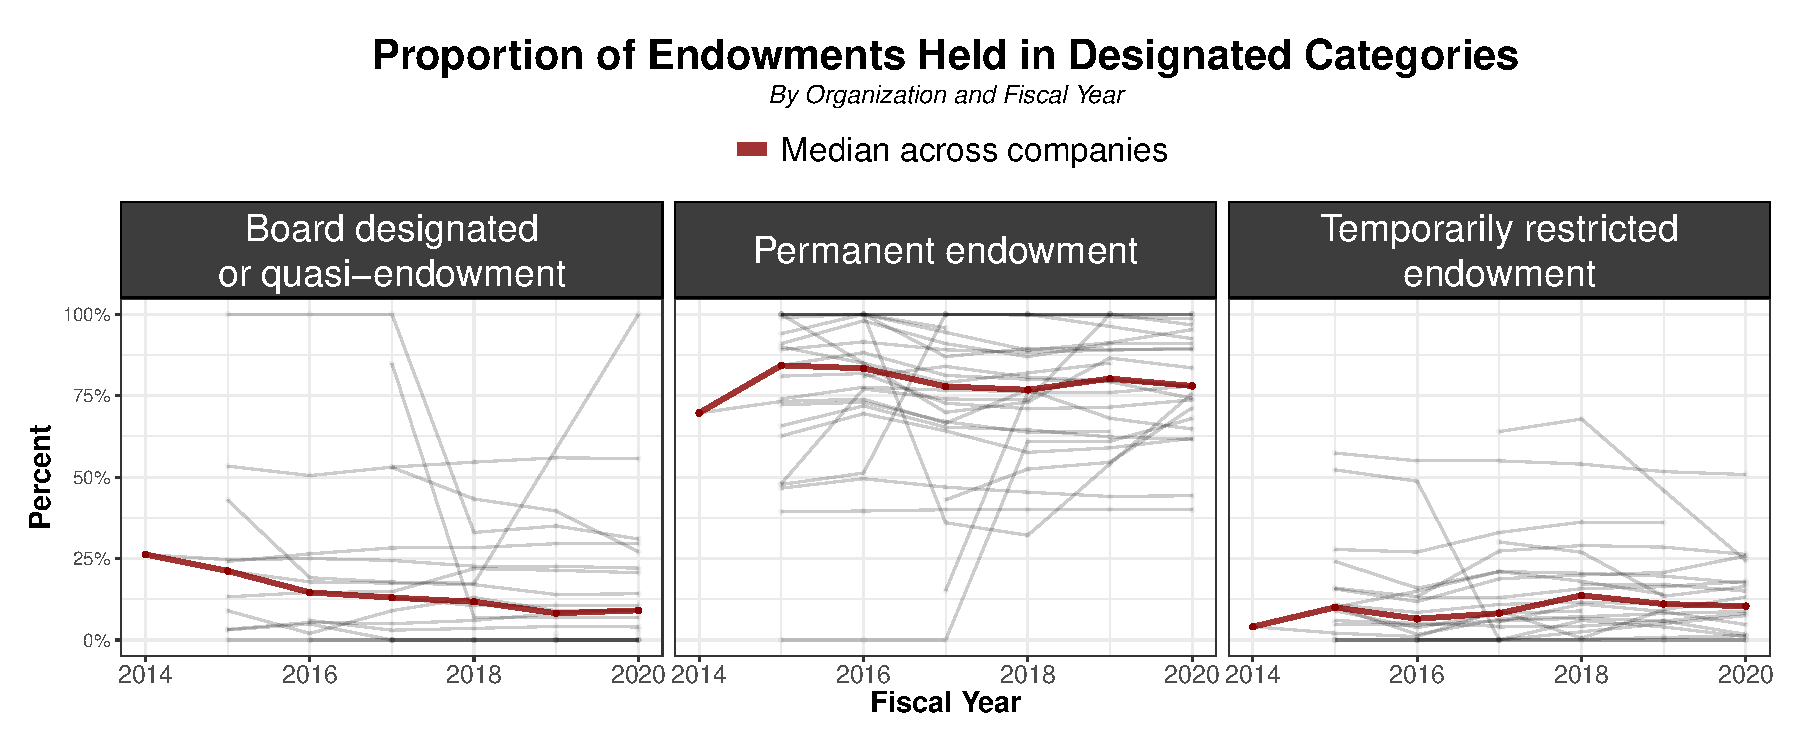
\includegraphics[width=1\linewidth,]{../images/proportion_endowment_categories} \caption{\label{fig:endowment-type}The percent of endowments held as a temporarily restricted endowment, permanent endowment, or board designated or quasi-endowment. The median across all companies by fiscal year is shown in red.}\label{fig:proportion-endowment-categories}
\end{figure}

However, there are several notable exceptions to the general trend of
consistency across years. Defining variability as the maximum standard
deviation of the proportions for each category, the most variable 5
companies were Fort Wayne Ballet, San Francisco Ballet, Nashville
Ballet, Atlanta Ballet, and the Washington Ballet (Figure
\ref{fig:prop-most-variable}).

\begin{itemize}
\tightlist
\item
  For Fort Wayne Ballet, most of the endowment funds (86\%) were board
  designated/quasi-endowment in 2017, but this dropped to a mere 7\% in
  2018. The percentage of the endowment funds in the permanent endowment
  category increased accordingly.
\item
  100\% of San Francisco Ballet's endowment was in the board
  designated/quasi-endowment category up until 2018, when the percentage
  in board designated/quasi-endowment dropped to 33\% and most (61\%)
  was a permanent endowment.
\item
  The trends in Nashville Ballet's endowment went the opposite
  direction, with a large increase in the percentage in the board
  designated/quasi-endowment category (17\% to 74\%) and decrease in the
  percentage in the permanent category.
\item
  For Atlanta Ballet, there is a dramatic shift in 2017 where the
  percentage held as temporarily restricted goes from 0\% to 64\%.
\item
  The Washington Ballet had a high proportion of its endowment in the
  temporarily restricted category (52\%) but by 2017 all their endowment
  funds were in the permanent endowment category.
\end{itemize}

\begin{figure}[H]
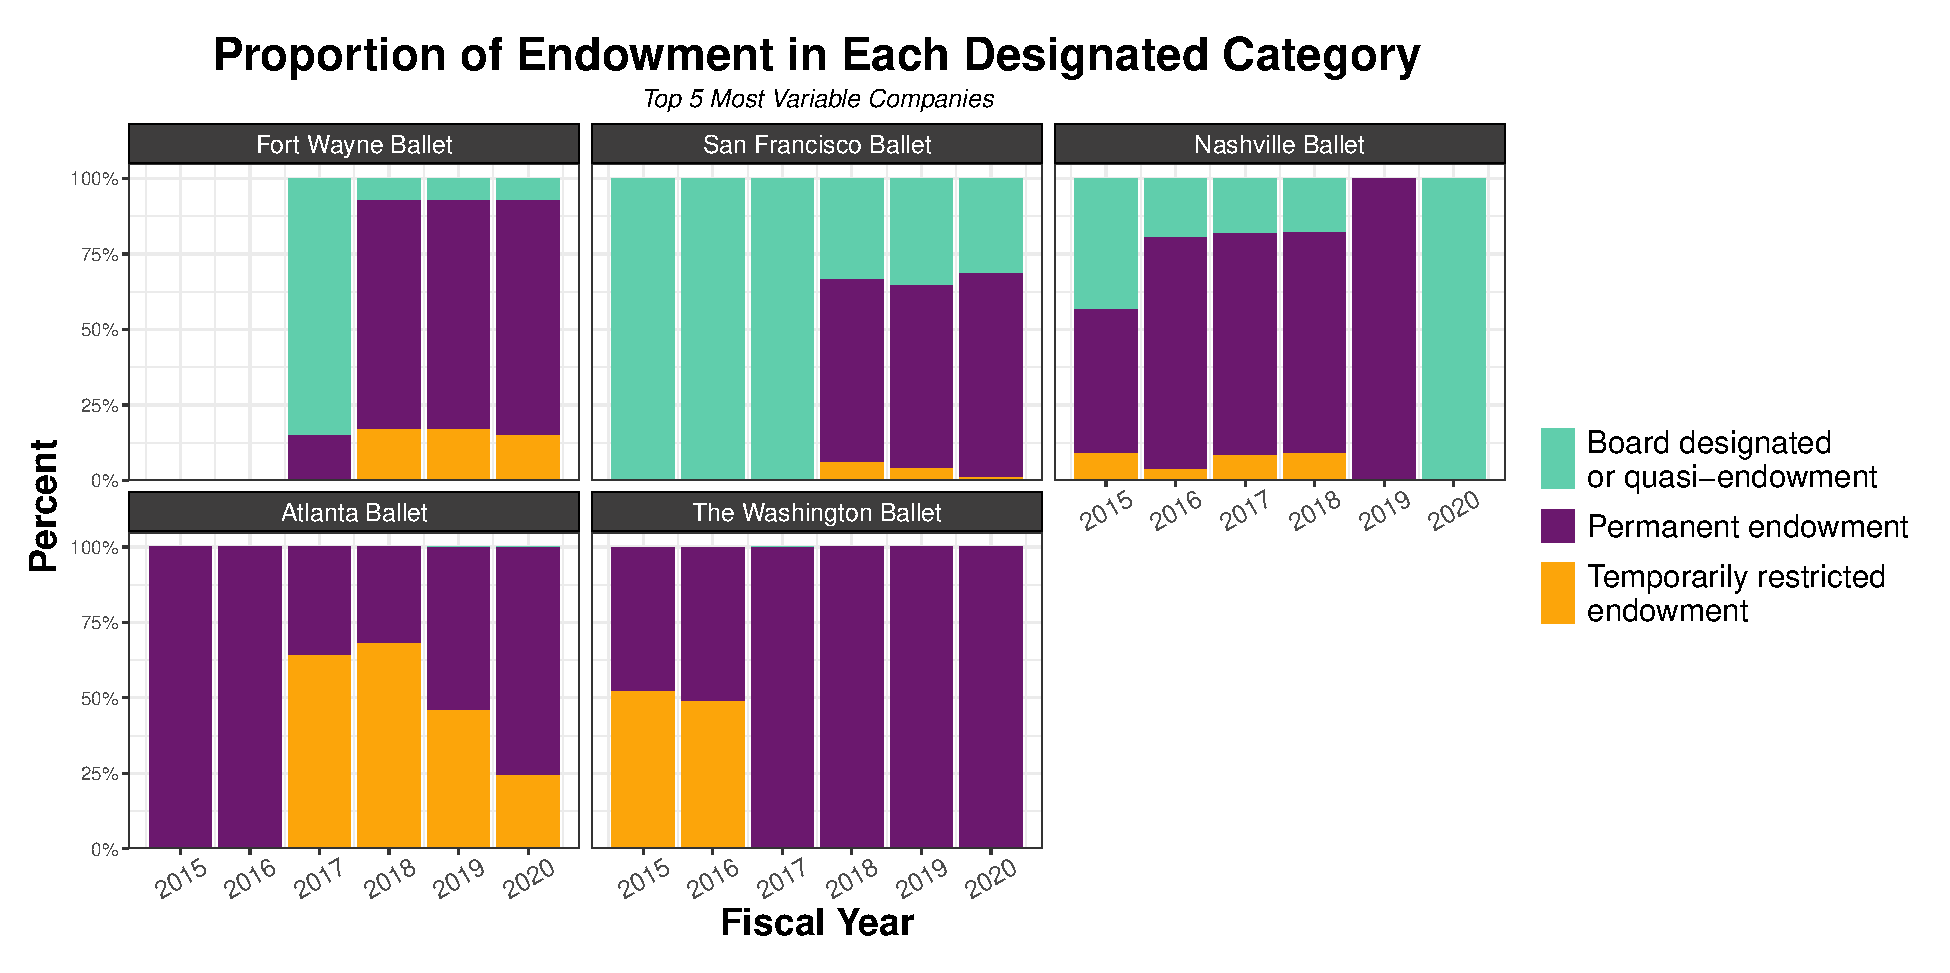
\includegraphics[width=1\linewidth,]{../images/prop_endowment_type_most_variable} \caption{\label{fig:prop-most-variable} Proportions of endowments in each designated category over time for the 5 companies with the most variability. We defined the most variable companies by considering the maximum standard deviation in the proportion in any one category.}\label{fig:proportion-endowment-categories-most-variable}
\end{figure}

\hypertarget{which-companies-have-endowments}{%
\subsubsection{Which Companies have
Endowments?}\label{which-companies-have-endowments}}

As we discuss these endowment analyses, one of the most fundamental
questions about endowments is how many companies report them, and how
that varies over time. To report endowments, nonprofits fill out
Schedule D in Form 990. Out of 169 dance companies we investigated, 47
reported endowments at least once in Schedule D (Table
\ref{table:filled-scheduled}).

\begin{table}[!h]

\caption{\label{tab:unnamed-chunk-2}Number of Companies that Reported an Endowment}
\centering
\begin{tabular}[t]{>{\raggedright\arraybackslash}p{10em}>{\raggedleft\arraybackslash}p{10em}>{\raggedleft\arraybackslash}p{10em}}
\toprule
 & Reported an Endowment & Did Not Report an Endowment\\
\midrule
\addlinespace[0.5em]
\multicolumn{3}{l}{\textbf{By Year}}\\
\hline
\hspace{1em}2014 & 6 & 1\\
\hspace{1em}2015 & 70 & 35\\
\hspace{1em}2016 & 79 & 37\\
\hspace{1em}2017 & 83 & 42\\
\hspace{1em}2018 & 96 & 40\\
\hspace{1em}2019 & 106 & 40\\
\hspace{1em}2020 & 83 & 40\\
\hspace{1em}2021 & 21 & 6\\
\addlinespace[0.5em]
\multicolumn{3}{l}{\textbf{\makecell[l]{Reported an Endowment\\at Least Once}}}\\
\hline
\hspace{1em} & 122 & 47\\
\bottomrule
\end{tabular}
\end{table}

\hypertarget{ranking-companies-endowments}{%
\subsubsection{Ranking Companies'
Endowments}\label{ranking-companies-endowments}}

Ranking companies can be useful to see how endomwents did relative to
each other rather than looking at the raw values, which are on immensely
different scales.

When we look at the rankings of the beginning of year balance of
companies' endowments, we see immediately that the top 7 companies, New
York City Ballet, San Francisco Ballet, Houston Ballet, Alvin Ailey
American Dance Theater, American Ballet Theatre, Pacific Northwest
Ballet, and Boston Ballet, see no changes in ranking from 2013 to 2020
(Figure \ref{fig:rank-endowments}) .

Below the top 7, there are more shifts in the rankings across time, with
some notable companies changing dramatically in ranking. This includes:

\begin{itemize}
\tightlist
\item
  A dramatic decrease in Aspen Santa Fe Ballet's ranking from 2018
  through 2020
\item
  A marked increase in:

  \begin{itemize}
  \tightlist
  \item
    Joffrey Ballet's ranking
  \item
    Orlando Ballet's ranking
  \item
    Fort Wayne Ballet's ranking
  \item
    Ballet Arizona's ranking
  \end{itemize}
\item
  A decrease in Atlanta Ballet's ranking from 2013 to 2015 that then
  recovered.
\end{itemize}

\begin{figure}[H]
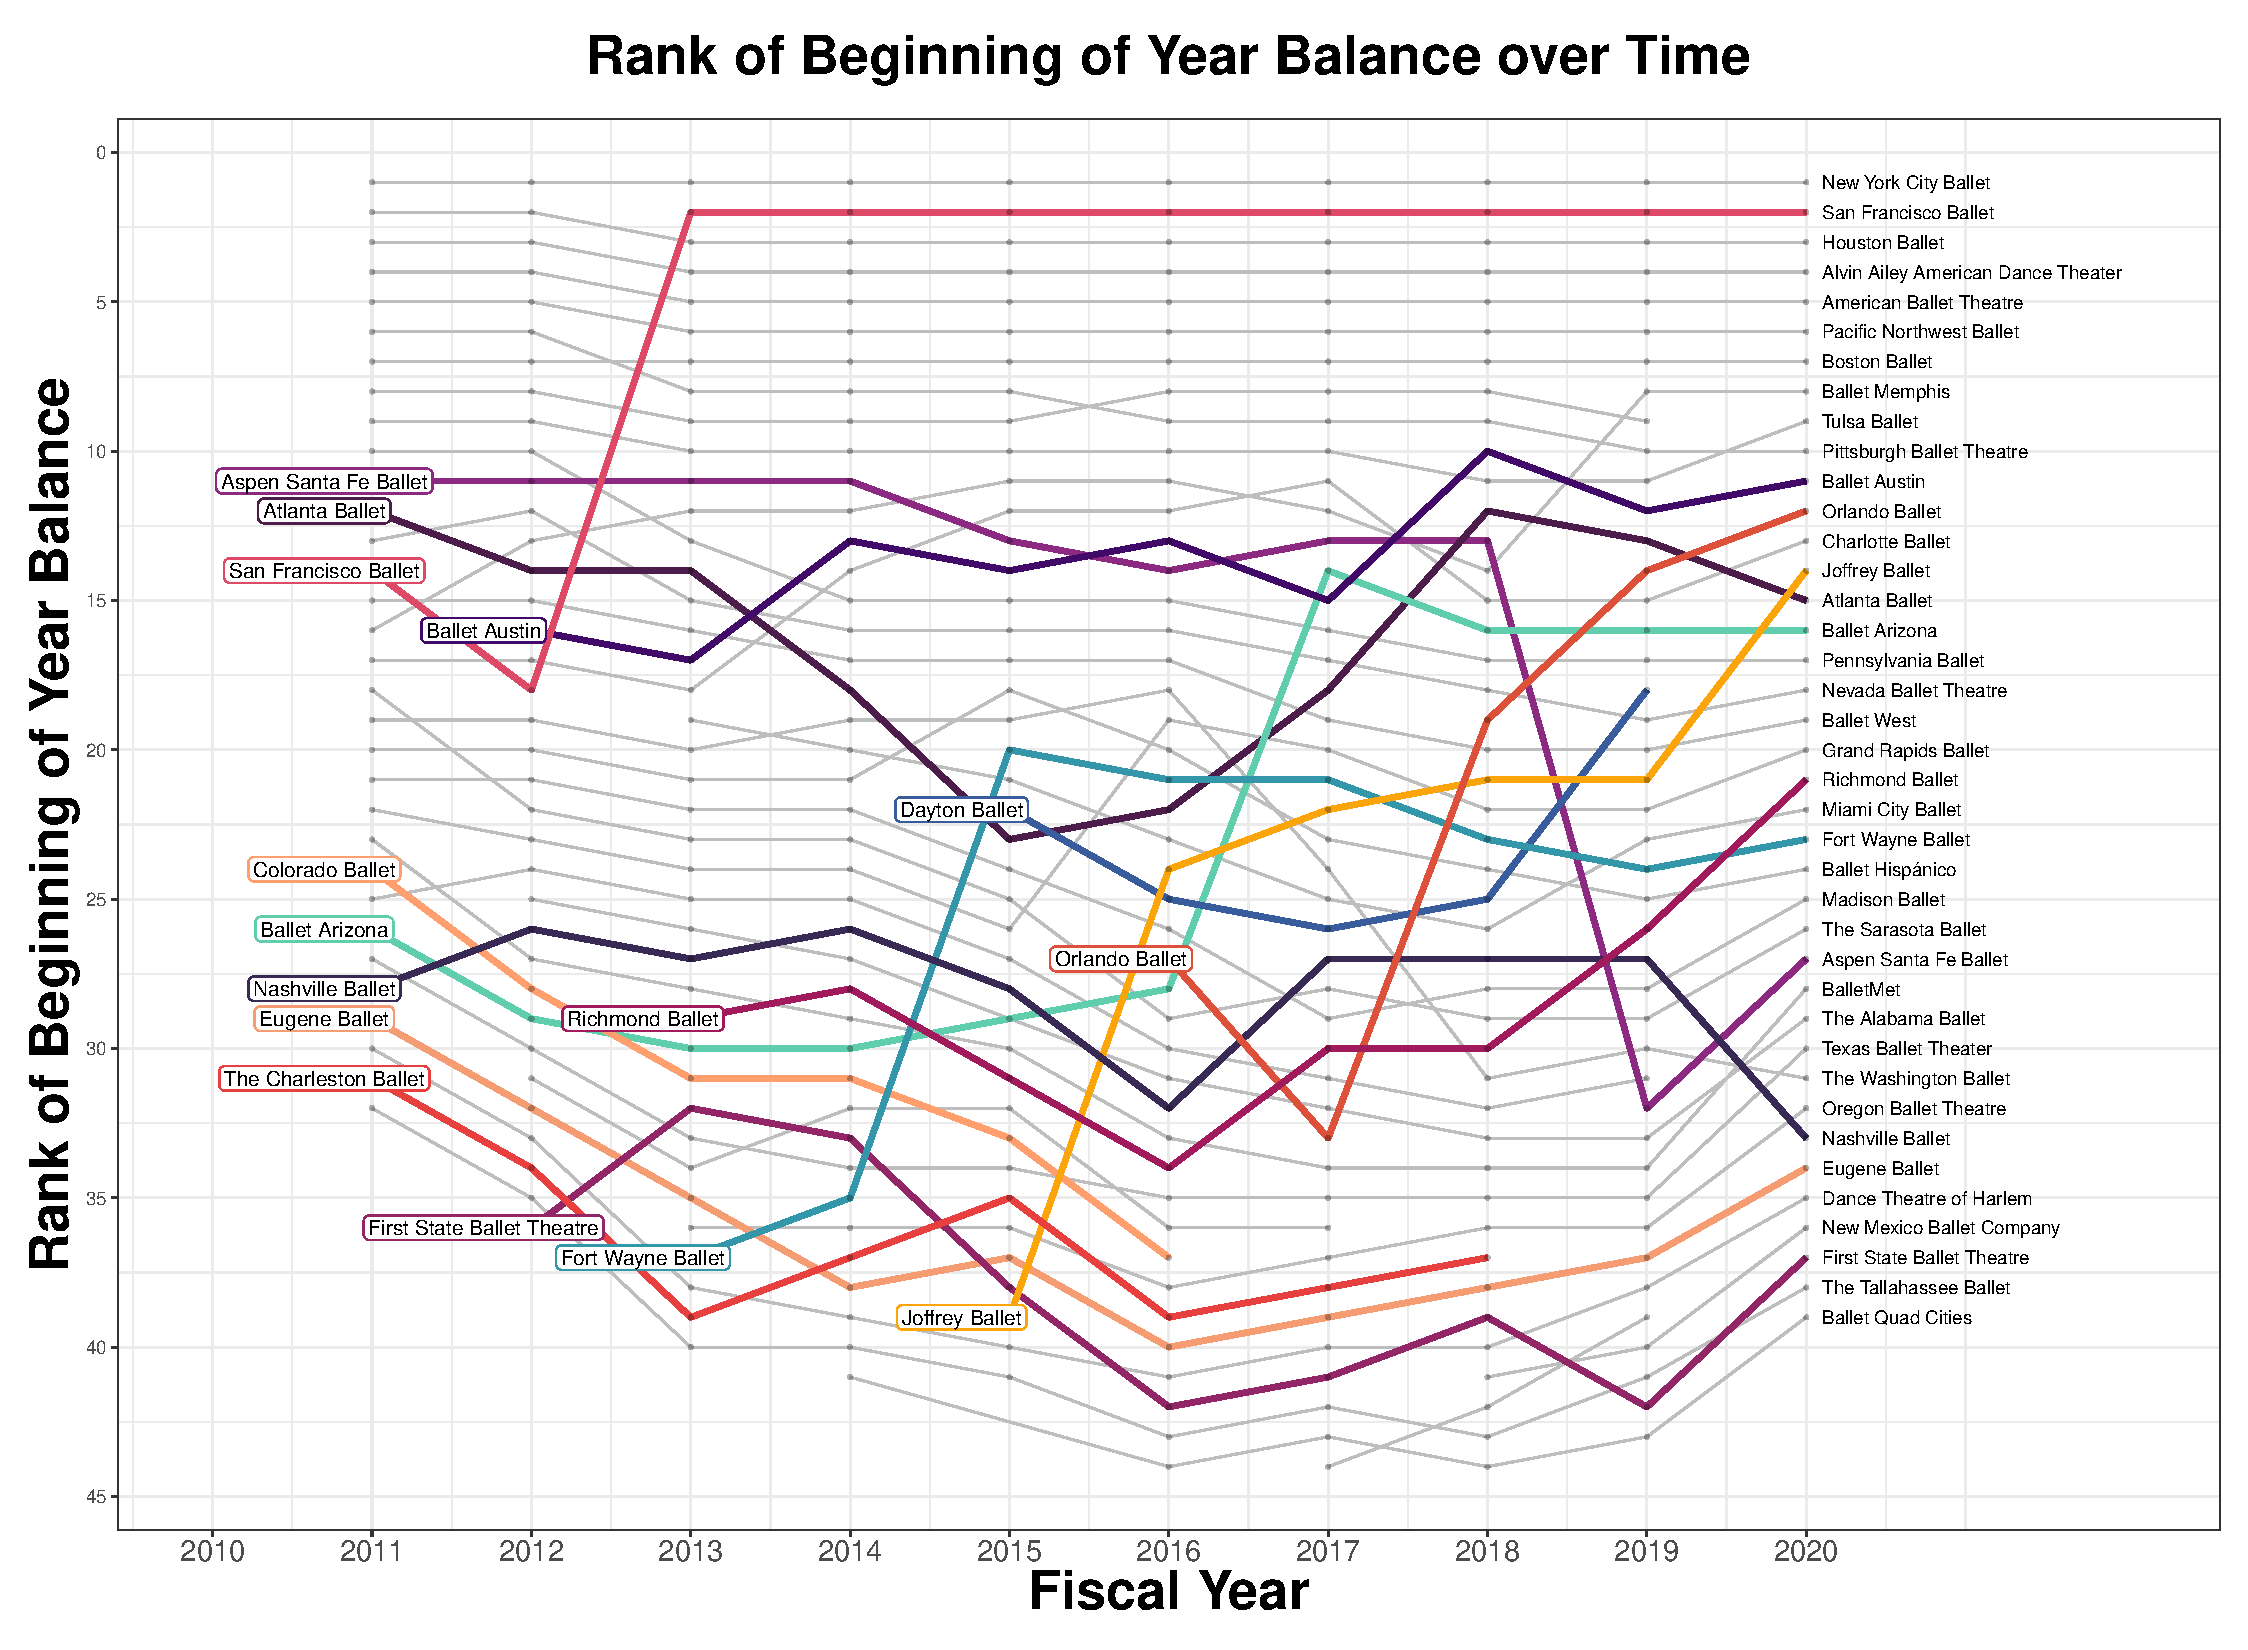
\includegraphics[width=1\linewidth,]{../images/rank_of_beginning_year_balance} \caption{\label{fig:rank-endowments}Rank of the endowment beginning of year balance over time. The 15 companies with the most variability in ranking, defined as the mean difference in rankings between fiscal years, are shown in color. Names of all companies are on the right.}\label{fig:rank-og-beginning-year-balance}
\end{figure}

When we add information on how these companies ranked in contributions
(Figure \ref{fig:rank-endowments-color-contribution}), we see that
although some organizations that are top ranked in endowment balance are
also top ranked in mean contributions, several of the companies that
experienced notable changes in their rankings also were ranked high in
contributions, in particular, Orlando Ballet and Joffrey Ballet.

\begin{figure}[H]
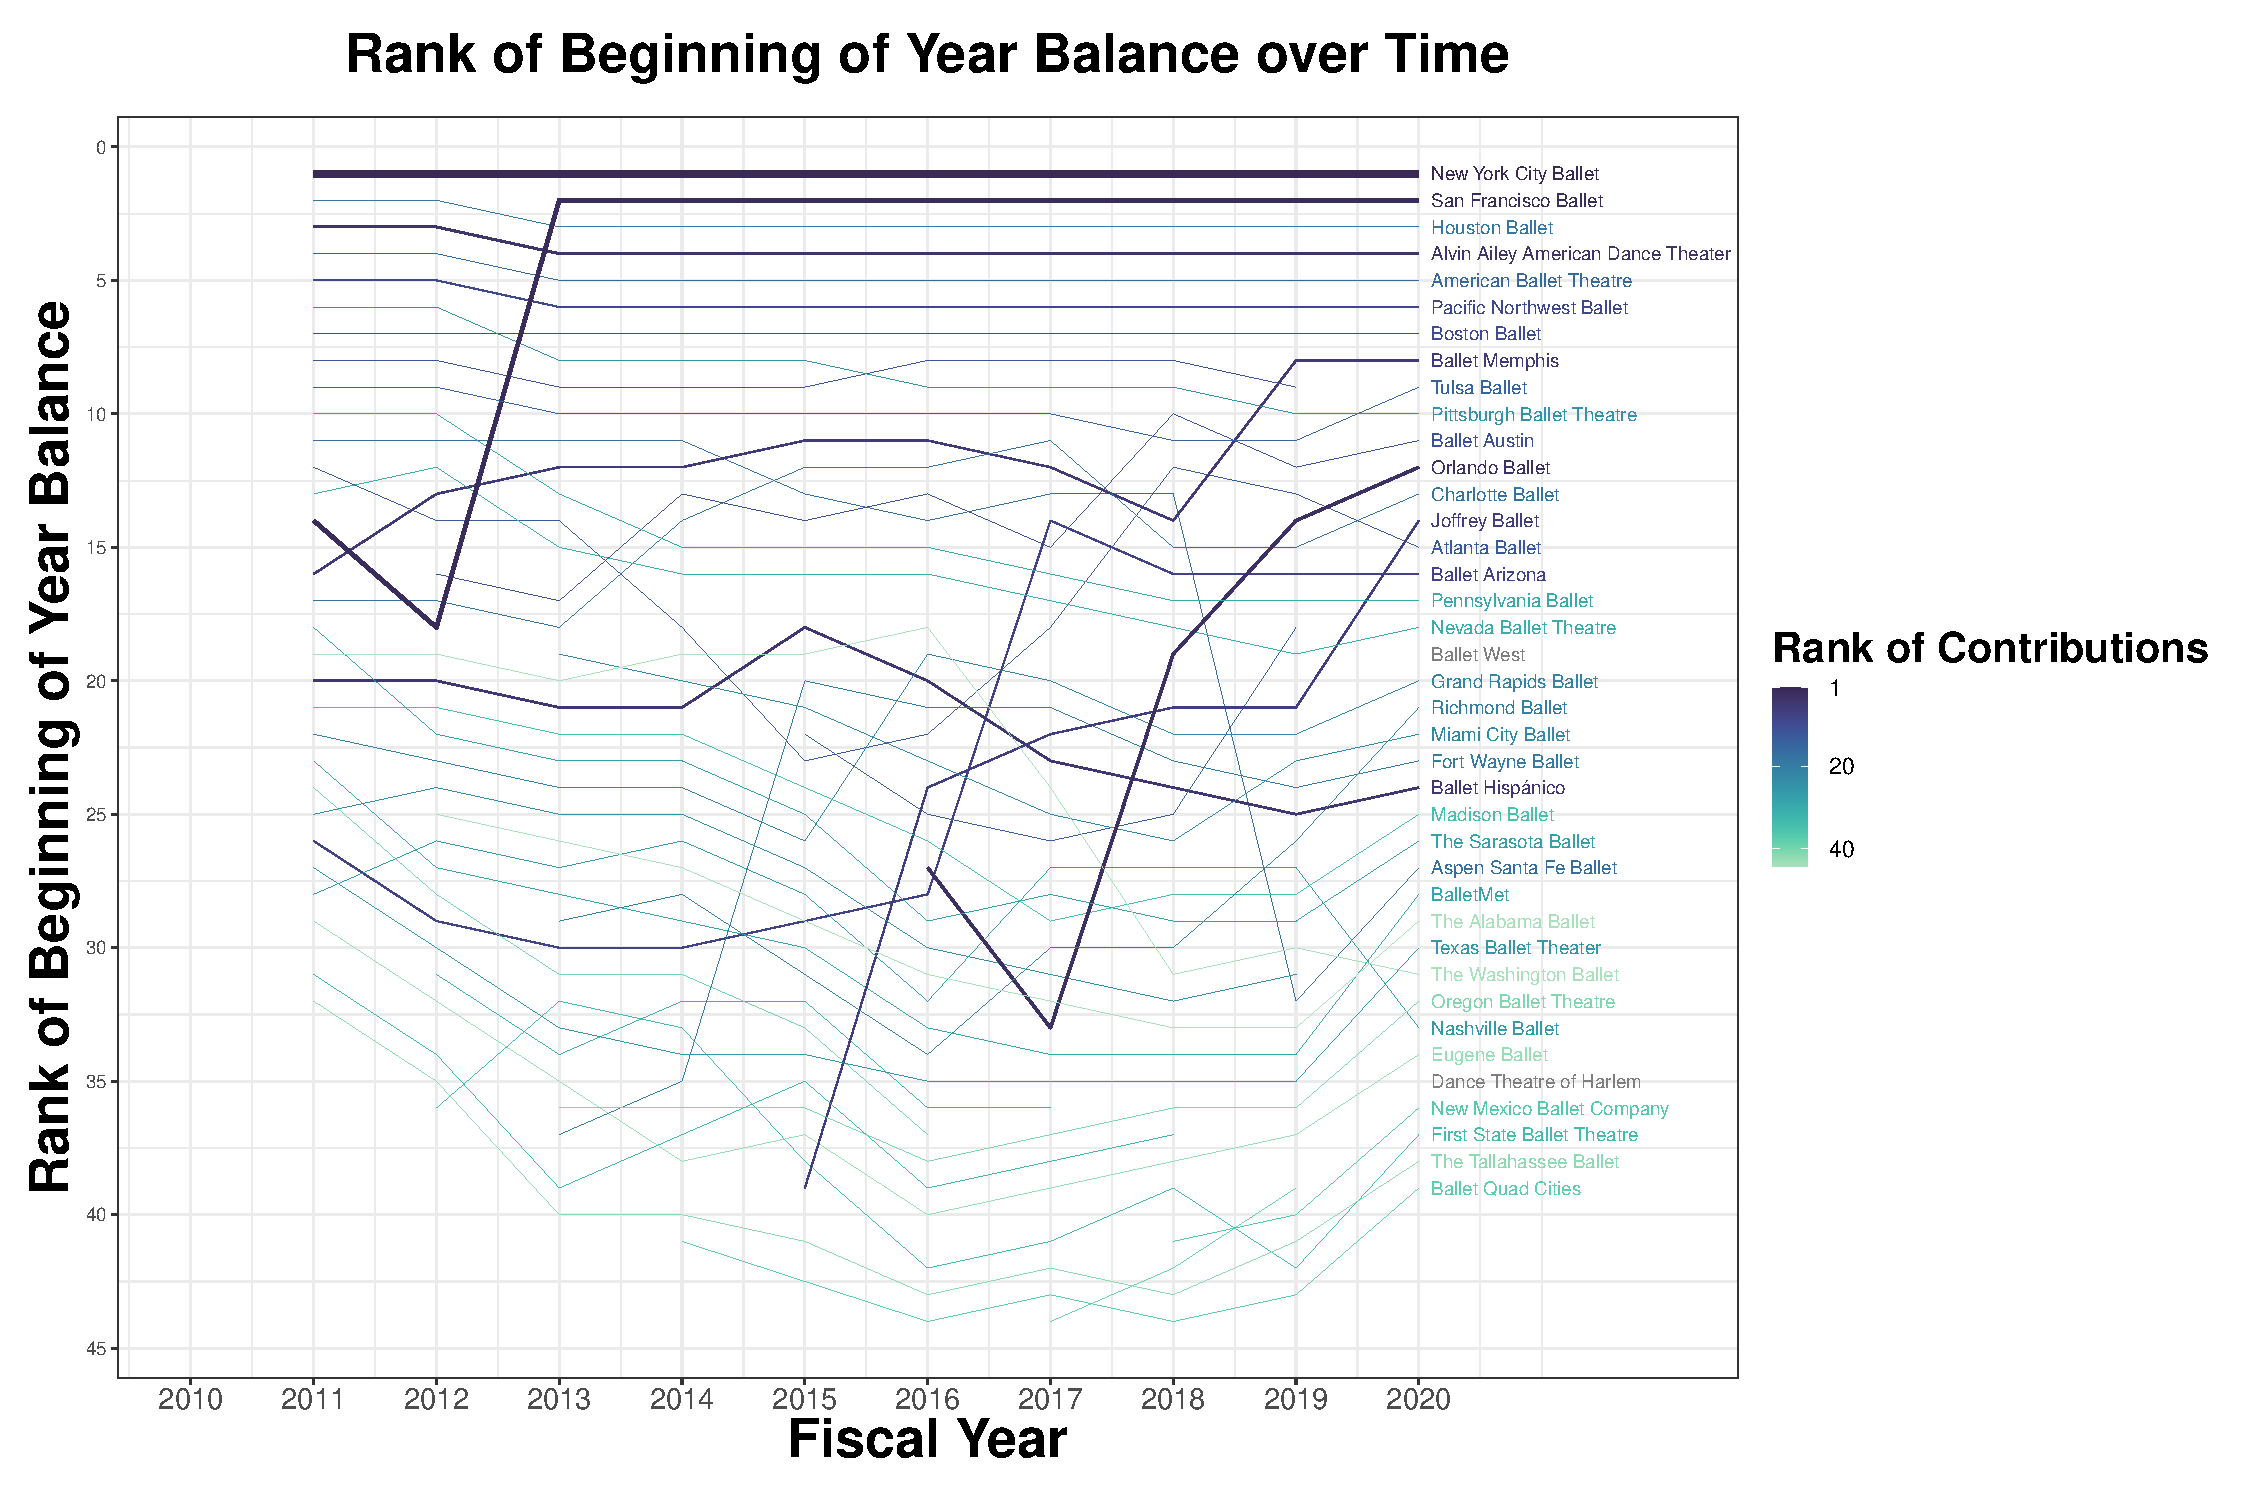
\includegraphics[width=1\linewidth,]{../images/rank-endowments-color-contribution} \caption{\label{fig:rank-endowments-color-contribution}Rank of the endowment beginning of year balance over time, where the color indicates the ranking of the mean contributions received over all years on file for the company.}\label{fig:unnamed-chunk-3}
\end{figure}

Looking more closely at the relationship between contribution rankings
and beginning of year balance rankings, in Figure \ref{fig:balancecont},
there is a strong relationship between how a company ranks with regard
to their contributions relative to the other companies and how a company
ranks in the endowment beginning of year balance. That is, when
companies are ranked high in the beginning of year balance, they tend to
rank high in contributions as well. As we would expect, this trend holds
across the full set of fiscal years considered.

However, the rankings are often not identical. If they were, all points
would fall on the red line, which represents an exact correspondence
between rankings. In some cases, a company consistently ranks higher in
contributions relative to the beginning of year balance. We summarize
whether the contributions or beginning of year balance tends to rank
higher for a given company in Figure \ref{fig:balancecontbar}. For
example, Ballet West ranked higher in the endowment beginning of year
balance for each year available (2016-2020), while Nashville Ballet
ranked higher in contributions than beginning of year balance for every
year on file (2011-2022).

\begin{figure}[H]
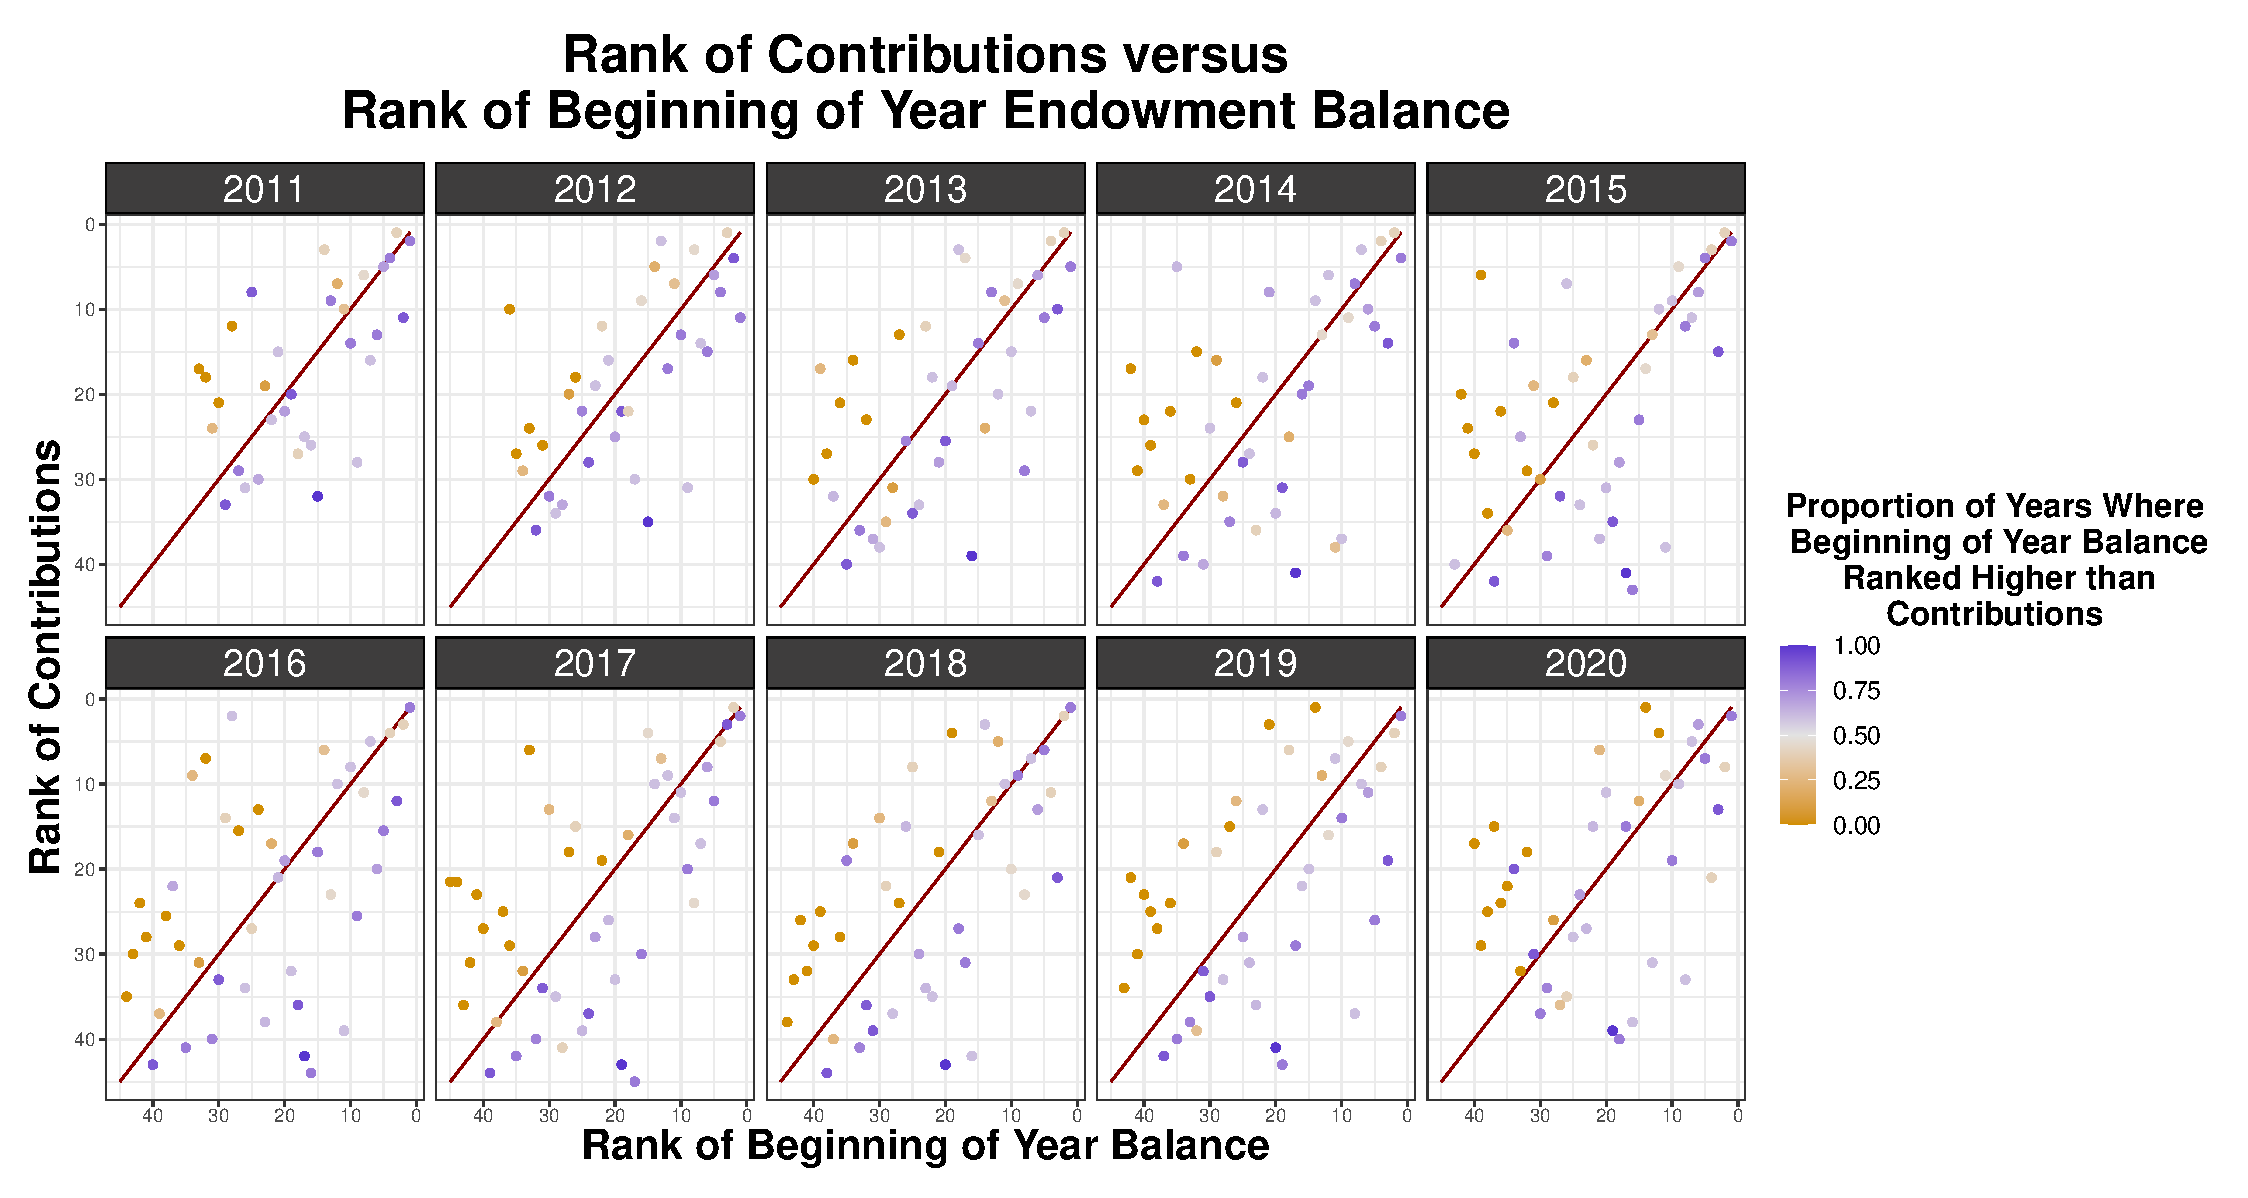
\includegraphics[width=0.75\linewidth,]{../images/compare-rankings-balance-contributions} \caption{\label{fig:balancecont} Comparing the rankings of beginning of year balance of the endowment to the ranking of contributions recieved.}\label{fig:compare-rankings-balance-contributions}
\end{figure}

\begin{figure}[H]
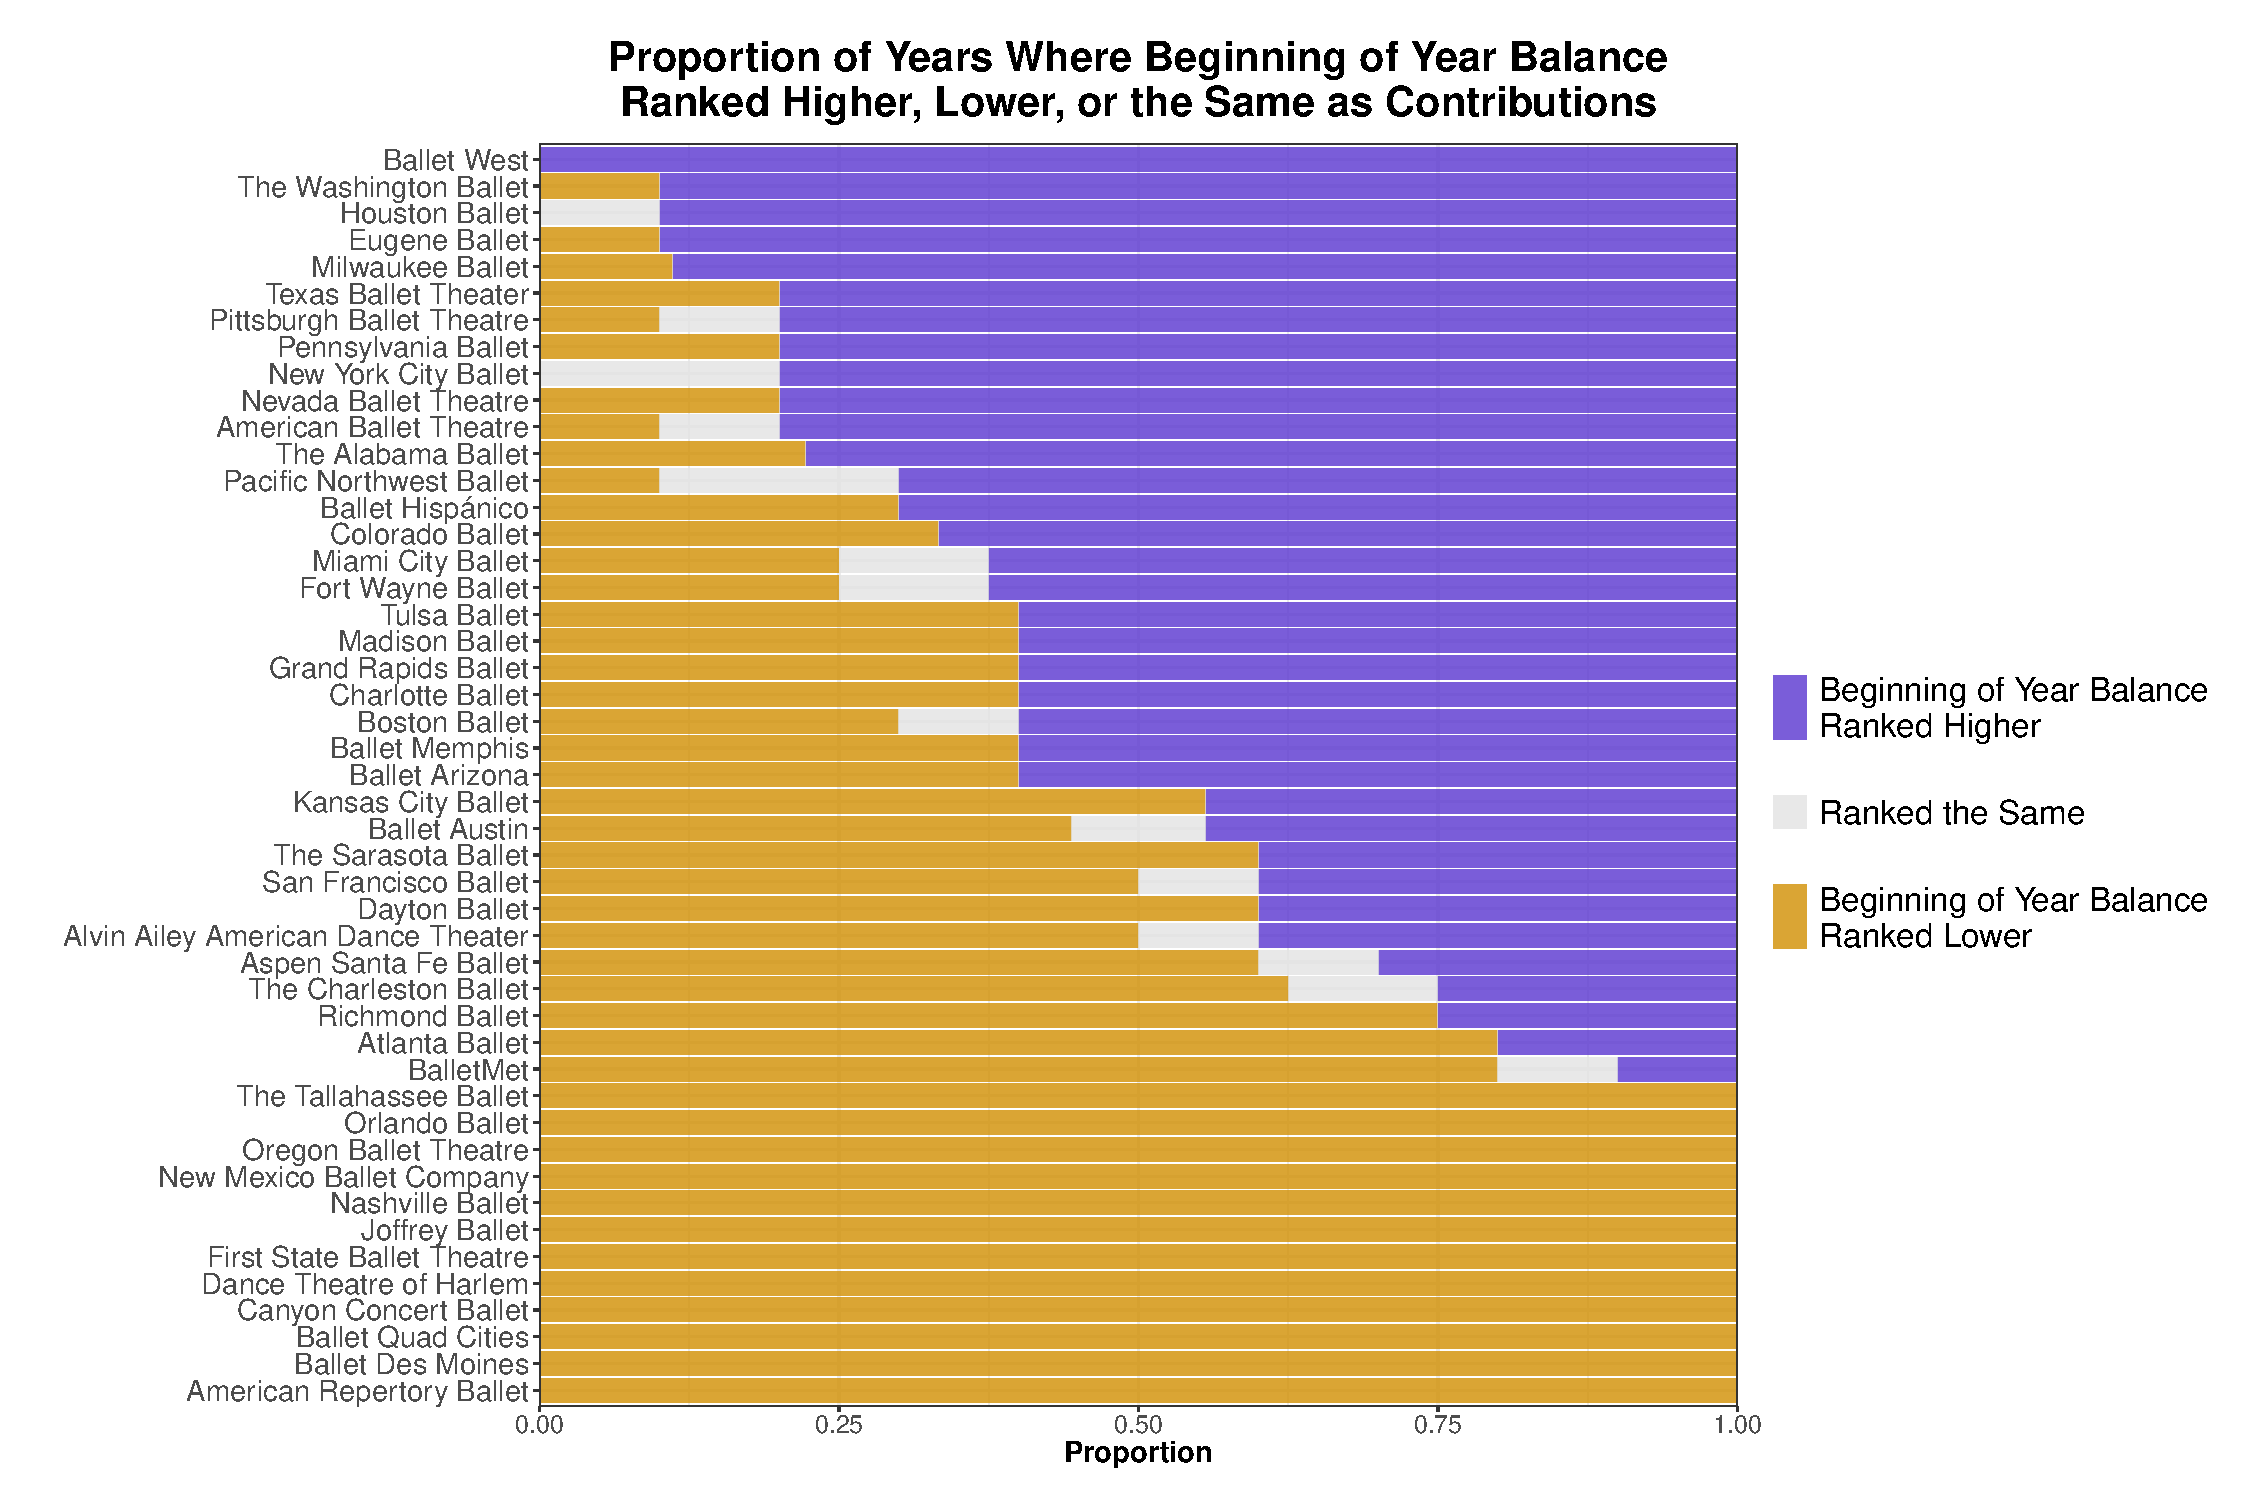
\includegraphics[width=0.6\linewidth,]{../images/compare-rankings-balance-contributions-barplot} \caption{\label{fig:balancecontbar} Comparing the proportion of years where a company ranked higher, lower, or the same in beginning of year balance compared to contributions received. A higher rank means a rank closer to 1, where 1 is the top possible rank.}\label{fig:compare-rankings-balance-contributions-barplot}
\end{figure}

% %%%%%%%%%%%%%%%%%%%%%%%%%%%%%%%%%%%%%%%%%%
% %% optional
% \supplementary{The following are available online at www.mdpi.com/link, Figure S1: title, Table S1: title, Video S1: title.}
%
% % Only for the journal Methods and Protocols:
% % If you wish to submit a video article, please do so with any other supplementary material.
% % \supplementary{The following are available at www.mdpi.com/link: Figure S1: title, Table S1: title, Video S1: title. A supporting video article is available at doi: link.}

\vspace{6pt}

%%%%%%%%%%%%%%%%%%%%%%%%%%%%%%%%%%%%%%%%%%
\acknowledgments{The authors thank the support and mentorship of
Dr.~Lindsay Poirier, Andrew Hoekstra, and Elizabeth Yntema.}

%%%%%%%%%%%%%%%%%%%%%%%%%%%%%%%%%%%%%%%%%%

%%%%%%%%%%%%%%%%%%%%%%%%%%%%%%%%%%%%%%%%%%
\conflictsofinterest{The authors declare no conflict of interest.}

%%%%%%%%%%%%%%%%%%%%%%%%%%%%%%%%%%%%%%%%%%
%% optional
\abbreviations{The following abbreviations are used in this manuscript:\\

\noindent
\begin{tabular}{@{}ll}
DDP & Dance Data Project \\
IRS & Internal Revenue Service \\
\end{tabular}}

\input{"appendix.tex"}

%%%%%%%%%%%%%%%%%%%%%%%%%%%%%%%%%%%%%%%%%%
% Citations and References in Supplementary files are permitted provided that they also appear in the reference list here.

%=====================================
% References, variant A: internal bibliography
%=====================================
%\reftitle{References}
%\begin{thebibliography}{999}
% Reference 1
%\bibitem[Author1(year)]{ref-journal}
%Author1, T. The title of the cited article. {\em Journal Abbreviation} {\bf 2008}, {\em 10}, 142--149.
% Reference 2
%\bibitem[Author2(year)]{ref-book}
%Author2, L. The title of the cited contribution. In {\em The Book Title}; Editor1, F., Editor2, A., Eds.; Publishing House: City, Country, 2007; pp. 32--58.
%\end{thebibliography}

% The following MDPI journals use author-date citation: Arts, Econometrics, Economies, Genealogy, Humanities, IJFS, JRFM, Laws, Religions, Risks, Social Sciences. For those journals, please follow the formatting guidelines on http://www.mdpi.com/authors/references
% To cite two works by the same author: \citeauthor{ref-journal-1a} (\citeyear{ref-journal-1a}, \citeyear{ref-journal-1b}). This produces: Whittaker (1967, 1975)
% To cite two works by the same author with specific pages: \citeauthor{ref-journal-3a} (\citeyear{ref-journal-3a}, p. 328; \citeyear{ref-journal-3b}, p.475). This produces: Wong (1999, p. 328; 2000, p. 475)

%=====================================
% References, variant B: external bibliography
%=====================================
\reftitle{References}
\externalbibliography{yes}
\bibliography{mybibfile.bib}

%%%%%%%%%%%%%%%%%%%%%%%%%%%%%%%%%%%%%%%%%%
%% optional

%% for journal Sci
%\reviewreports{\\
%Reviewer 1 comments and authors’ response\\
%Reviewer 2 comments and authors’ response\\
%Reviewer 3 comments and authors’ response
%}

%%%%%%%%%%%%%%%%%%%%%%%%%%%%%%%%%%%%%%%%%%


\end{document}
